\section{Holographie}
Man kann die Kohärenzlänge $l_k$ des Lasers wie folgt bestimmen:
\begin{equation}
    l_k=\tau_k\cdot\frac{c}{n}\frac{c}{\left(\Delta\nu\right)_\text{Verst}}
\end{equation}
Mit den Ergebnissen aus dem Kapitel 'Axiale Lasermoden' folgt:
\begin{equation}
    l_k=\left(0,491\pm0,003\right)\,\text{m}
\end{equation}
Mit dem Laser in unserem Versuchsaufbau können wir ein Hologramm sichtbar machen.
Dazu wird der Strahl mit einer Linse ausgeweitet und das Hologramm (eine Platte, auf der das Bild gespeichert ist) beleuchtet.\\
Dabei konnten wir folgendes Bild erkennen:
\begin{figure}[h]
    \centering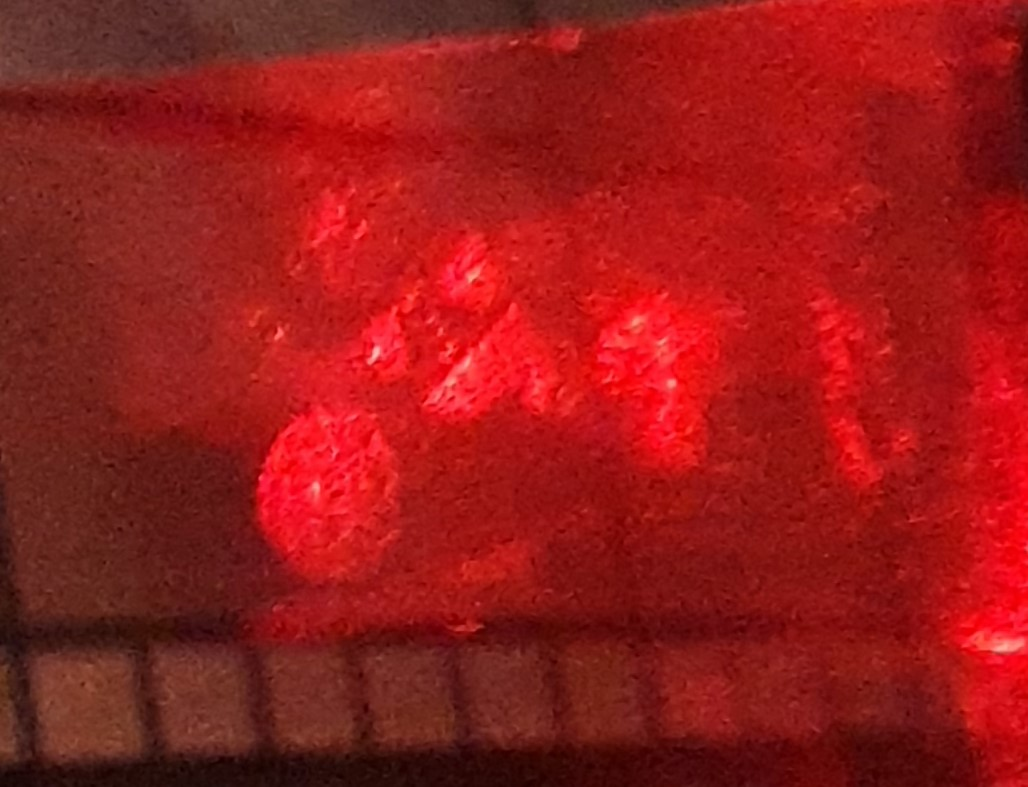
\includegraphics[width=0.5\textwidth]{Auswertung-Dominik/hologramm.jpg}
    \caption{Aufgenommenes Hologramm}
\end{figure}\\
Zu erkennen war ein Fußballspielender Schlumpf.
Auf dem aufgenommenen Foto ist dies leider nicht so gut erkennbar, man kann aber jedoch den Fußball erahnen. Durch bewegen des Kopfes konnten wir während dem Versuch auch die verschiedenen Fassetten des Hologramms wahrnehmen.
